\documentclass[12pt]{book}

\newcommand{\thetitle}{Think Java: How to Think Like a Computer Scientist}
\title{\thetitle}

\newcommand{\theauthors}{Allen Downey and Chris Mayfield}
\author{\theauthors}

\newcommand{\theversion}{Version 6.0 Draft -- \today}
\date{\theversion}

\usepackage{geometry}
\geometry{
    width=5.5in,
    height=8.5in,
    hmarginratio=3:2,
    vmarginratio=1:1,
    includehead=true,
    headheight=15pt
}

% paragraph spacing
\setlength{\parindent}{0pt}                      % 17.62482pt
\setlength{\parskip}{12pt plus 4pt minus 4pt}    % 0.0pt plus 1.0pt
\linespread{1.05}
\def\arraystretch{1.5}

% list spacing
\setlength{\topsep}{5pt plus 2pt minus 3pt}      % 10.0pt plus 4.0pt minus 6.0pt
\setlength{\partopsep}{-6pt plus 2pt minus 2pt}  %  3.0pt plus 2.0pt minus 2.0pt
\setlength{\itemsep}{0pt}                        %  5.0pt plus 2.5pt minus 1.0pt

% these are copied from tex/latex/base/book.cls
% all I changed is afterskip
\makeatletter
\renewcommand{\section}{\@startsection {section}{1}{\z@}%
    {-3.5ex \@plus -1ex \@minus -.2ex}%
    {0.7ex \@plus.2ex}%
    {\normalfont\Large\bfseries}}
\renewcommand\subsection{\@startsection{subsection}{2}{\z@}%
    {-3.25ex\@plus -1ex \@minus -.2ex}%
    {0.3ex \@plus .2ex}%
    {\normalfont\large\bfseries}}
\renewcommand\subsubsection{\@startsection{subsubsection}{3}{\z@}%
    {-3.25ex\@plus -1ex \@minus -.2ex}%
    {0.3ex \@plus .2ex}%
    {\normalfont\normalsize\bfseries}}
\makeatother

% table of contents vertical spacing
\usepackage{tocloft}
\setlength\cftparskip{8pt plus 4pt minus 4pt}

% The following line adds a little extra space to the column
% in which the Section numbers appear in the table of contents
\makeatletter
\renewcommand{\l@section}{\@dottedtocline{1}{1.5em}{3.0em}}
\makeatother

% customize page headers
\usepackage{fancyhdr}
\pagestyle{fancyplain}
\renewcommand{\chaptermark}[1]{\markboth{Chapter \thechapter ~~ #1}{}}
\renewcommand{\sectionmark}[1]{\markright{\thesection ~~ #1}}
\lhead[\fancyplain{}{\bfseries\thepage}]%
      {\fancyplain{}{\bfseries\rightmark}}
\rhead[\fancyplain{}{\bfseries\leftmark}]%
      {\fancyplain{}{\bfseries\thepage}}
\cfoot{}
%\rfoot{\textcolor{gray}{\tiny ThinkJava Draft \today}}

% balanced index with TOC entry
\usepackage{makeidx}
\makeindex
%\usepackage[totoc]{idxlayout}

% automatically index glossary terms
\newcommand{\term}[1]{%
\index{#1}
\item[#1:]}
% TODO: doesn't work with plastex
%\newcommand{\term}[1]{\item[#1:]}

% where to find graphics
\usepackage{graphicx}
%\graphicspath{{figs/}}

%% tweak spacing of figures and captions
%\usepackage{floatrow}
%\usepackage{caption}
%\captionsetup{
%    font=small,
%    labelformat=empty,
%    justification=centering,
%    skip=4pt
%}

% format end of chapter excercises
\usepackage{amsmath}
\usepackage{amsthm}
\newtheoremstyle{exercise}
  {12pt}        % space above
  {12pt}        % space below
  {}            % body font
  {}            % indent amount
  {\bfseries}   % head font
  {}            % punctuation
  {12pt}        % head space
  {}            % custom head
\theoremstyle{exercise}
\newtheorem{exercise}{Exercise}[chapter]

% colors for code listings and output
\usepackage{xcolor}
\definecolor{bgcolor}{HTML}{FAFAFA}
\definecolor{comment}{HTML}{007C00}
\definecolor{keyword}{HTML}{0000FF}
\definecolor{strings}{HTML}{B20000}

% syntax highlighting in code listings
\usepackage{textcomp}
\usepackage{listings}
\lstset{
    language=java,
    basicstyle=\ttfamily,
    backgroundcolor=\color{bgcolor},
    commentstyle=\color{comment},
    keywordstyle=\color{keyword},
    stringstyle=\color{strings},
    columns=fullflexible,
    keepspaces=true,
    showstringspaces=false,
    upquote=true,
    aboveskip=\parskip,
    belowskip=\parskip
}

% code listing environments
\lstnewenvironment{code}
{\minipage{\linewidth}}
{\endminipage}
\lstnewenvironment{stdout}
{\lstset{commentstyle=,keywordstyle=,stringstyle=}\minipage{\linewidth}}
{\endminipage}

% pdf hyperlinks, table of contents, and document properties
\usepackage[pdftex]{hyperref}
\hypersetup{%
  pdftitle={\thetitle},
  pdfauthor={\theauthors},
  pdfsubject={\theversion},
  pdfkeywords={},
  bookmarksopen=false,
  colorlinks=true,
  citecolor=black,
  filecolor=black,
  linkcolor=black,
  urlcolor=blue
}

% inline syntax formatting
\newcommand{\java}[1]{\lstinline{#1}} %\end{
%\newcommand{\java}[1]{\verb"#1"}
%\newcommand{\java}[1]{{\tt #1}}

\begin{document}
\setcounter{chapter}{6}

\chapter{Loops and iteration}

TODO

\section{Multiple assignment}
\index{assignment}
\index{statement!assignment}
\index{multiple assignment}

%TODO move to chapter 5

You can make more than one assignment to the same variable;
the effect is to replace the old value with the new.

\begin{code}
    int liz = 5;
    System.out.print(liz);
    liz = 7;
    System.out.println(liz);
\end{code}

The output of this program is {\tt 57}, because the first
time we print {\tt liz} her value is 5, and the second time
her value is 7.

This kind of {\bf multiple assignment} is the reason I
described variables as a {\em container} for values.  When
you assign a value to a variable, you change the contents of
the container, as shown in the figure:


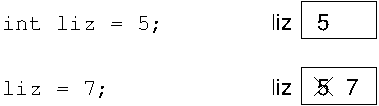
\includegraphics{figs/assign2.pdf}


When there are multiple assignments to a variable, it is especially
important to distinguish between an assignment statement and a
statement of equality.  Because Java uses the {\tt =} symbol for
assignment, it is tempting to interpret a statement like {\tt a = b}
as a statement of equality.  It is not!

First of all, equality is commutative, and assignment is not.
For example, in mathematics if $a = 7$ then $7 = a$.  But in
Java {\tt a = 7;} is a legal assignment statement, and {\tt 7 = a;}
is not.

Furthermore, in mathematics, a statement of equality is true
for all time.  If $a = b$ now, then $a$ will always equal $b$.
In Java, an assignment statement can make two variables equal,
but they don't have to stay that way!

\begin{code}
    int a = 5;
    int b = a;     // a and b are now equal
    a = 3;         // a and b are no longer equal
\end{code}

The third line changes the value of {\tt a} but it does not
change the value of {\tt b}, so they are no longer equal.
In some programming languages a different symbol is used
for assignment, such as {\tt <-} or {\tt :=}, to
avoid this confusion.

Although multiple assignment is frequently useful, you should use it
with caution.  If the values of variables change often, it can make
the code difficult to read and debug.


\section{The {\tt while} statement}
\index{statement!while}
\index{while statement}
\index{iteration}

Computers are often used to automate repetitive tasks.  Repeating
tasks without making errors is something that
computers do well and people do poorly.

We have already seen methods like {\tt countdown} and {\tt factorial}
that use recursion to perform repetition. This process is also called
{\bf iteration}. Java provides language features that make
it easier to write these methods.
In this chapter we are going to look at the {\tt while} statement.
Later on (in Section~\ref{for}) will check out the {\tt for} statement.

Using a {\tt while} statement, we can rewrite {\tt countdown}:

\begin{code}
  public static void countdown(int n) {
    while (n > 0) {
      System.out.println(n);
      n = n-1;
    }
    System.out.println("Blastoff!");
  }
\end{code}

You can almost read a {\tt while} statement like
English.  What this means is, ``While {\tt n} is greater than
zero, print the value of {\tt n} and then reduce
the value of {\tt n} by 1.  When you get to zero, print the
word `Blastoff!'''

More formally, the flow of execution for a {\tt while} statement
is as follows:

\begin{enumerate}

\item Evaluate the condition in parentheses, yielding {\tt true}
or {\tt false}.

\item If the condition is false, exit the {\tt while} statement
and continue execution at the next statement.

\item If the condition is true, execute the statements
between the squiggly-brackets, and then go back to step 1.

\end{enumerate}

This type of flow is called a {\bf loop} because the third step loops
back around to the top.  The statements inside the loop are called
the {\bf body} of the loop.
If the condition is false the
first time through the loop, the statements inside the loop are
never executed.

\index{loop}
\index{loop!body}
\index{loop!infinite}
\index{body!loop}
\index{infinite loop}

The body of the loop should change the value of
one or more variables so that, eventually, the condition becomes
false and the loop terminates.  Otherwise the loop will repeat
forever, which is called an {\bf infinite} loop.  An endless
source of amusement for computer scientists is the observation
that the directions on shampoo, ``Lather, rinse, repeat,'' are
an infinite loop.

In the case of {\tt countdown}, we can prove that the loop
terminates if {\tt n} is positive.
%
In other cases it is not so easy to tell:

\begin{code}
  public static void sequence(int n) {
    while (n != 1) {
      System.out.println(n);
      if (n%2 == 0) {           // n is even
        n = n / 2;
      } else {                  // n is odd
        n = n*3 + 1;
      }
    }
  }
\end{code}

The condition for this loop is {\tt n != 1}, so the loop
will continue until {\tt n} is 1, which will make the condition
false.

At each iteration, the program prints the value of {\tt n} and then
checks whether it is even or odd.  If it is even, the value of
{\tt n} is divided by two.  If it is odd, the value is replaced
by $3n+1$.  For example, if the starting value (the argument passed
to {\tt sequence}) is 3, the resulting sequence is
3, 10, 5, 16, 8, 4, 2, 1.

Since {\tt n} sometimes increases and sometimes decreases, there is no
obvious proof that {\tt n} will ever reach 1, or that the program will
terminate.  For some particular values of {\tt n}, we can prove
termination.  For example, if the starting value is a power of two, then
the value of {\tt n} will be even every time through the loop, until
we get to 1.  The previous example ends with such a sequence,
starting with 16.

Particular values aside, the interesting question is whether
we can prove that this program terminates for {\em all} values of n.
So far, no one has been able to prove it {\em or} disprove it!
For more information, see \url{http://en.wikipedia.org/wiki/Collatz_conjecture}.


\section{Generating tables}
\index{table}
\index{logarithm}

One of the things loops are good for is generating and printing
tabular data.  For example, before computers were readily
available, people had to calculate logarithms,
sines and cosines, and other common mathematical functions
by hand.

To make that easier, there were books containing long tables
where you could find the values of various functions.
Creating these tables was slow and boring, and the results
were full of errors.

When computers appeared on the scene, one of the initial reactions
was, ``This is great!  We can use the computers to generate the
tables, so there will be no errors.''  That turned out to be true
(mostly), but shortsighted.  Soon thereafter computers were so
pervasive that the tables became obsolete.

Well, almost.  For some operations, computers use tables of values to
get an approximate answer, and then perform computations to improve
the approximation.  In some cases, there have been errors in the
underlying tables, most famously in the table the original Intel
Pentium used to perform floating-point division\footnote{See
  \url{http://en.wikipedia.org/wiki/Pentium_FDIV_bug}.}.

\index{division!floating-point}

Although a ``log table'' is not as useful as it once was, it still
makes a good example of iteration.  The following program prints a
sequence of values in the left column and their logarithms in the
right column:

\begin{code}
    double x = 1.0;
    while (x < 10.0) {
      System.out.println(x + "   " + Math.log(x));
      x = x + 1.0;
    }
\end{code}

The output of this program is

\begin{stdout}
1.0   0.0
2.0   0.6931471805599453
3.0   1.0986122886681098
4.0   1.3862943611198906
5.0   1.6094379124341003
6.0   1.791759469228055
7.0   1.9459101490553132
8.0   2.0794415416798357
9.0   2.1972245773362196
\end{stdout}

Looking at these values, can you tell what base the {\tt log}
method uses?

Since powers of two are important
in computer science, we often want logarithms with
respect to base 2.  To compute them, we can use the formula:

\begin{equation*}
\log_2 x = log_e x / log_e 2
\end{equation*}

Changing the {\tt print} statement to

\begin{code}
      System.out.println(x + "   " + Math.log(x) / Math.log(2.0));
\end{code}

yields

\begin{stdout}
1.0   0.0
2.0   1.0
3.0   1.5849625007211563
4.0   2.0
5.0   2.321928094887362
6.0   2.584962500721156
7.0   2.807354922057604
8.0   3.0
9.0   3.1699250014423126
\end{stdout}

We can see that 1, 2, 4 and 8 are powers of two, because
their logarithms base 2 are round numbers.  If we wanted to find
the logarithms of other powers of two, we could modify the
program like this:

\begin{code}
    double x = 1.0;
    while (x < 100.0) {
      System.out.println(x + "   " + Math.log(x) / Math.log(2.0));
      x = x * 2.0;
    }
\end{code}

Now instead of adding something to {\tt x} each time through
the loop, which yields an arithmetic sequence, we multiply
{\tt x} by something, yielding a {\bf geometric} sequence.
The result is:

\begin{stdout}
1.0   0.0
2.0   1.0
4.0   2.0
8.0   3.0
16.0   4.0
32.0   5.0
64.0   6.0
\end{stdout}

Log tables may not be useful any more, but for computer scientists,
knowing the powers of two is!  When you have an idle
moment, you should memorize the powers of two up to 65536
(that's $2^{16}$).


\section{Encapsulation and generalization}
\label{encapsulation}

Encapsulation means taking a piece of code and wrapping it up
in a method, allowing you to take advantage of all the things methods
are good for.  We have seen two examples of encapsulation, when we
wrote {\tt printParity} in Section~\ref{alternative} and {\tt
isSingleDigit} in Section~\ref{boolean}.

Generalization means taking something specific, like printing
multiples of 2, and making it more general, like printing the
multiples of any integer.
\index{encapsulation}
\index{generalization}

Here's a method that encapsulates the loop from the previous
section and generalizes it to print multiples of {\tt n}.

\begin{code}
  public static void printMultiples(int n) {
    int i = 1;
    while (i <= 6) {
      System.out.print(n*i + "   ");
      i = i + 1;
    }
    System.out.println("");
  }
\end{code}

To encapsulate, all I had to do was add the first line,
which declares the name, parameter,
and return type.  To generalize, all I had to do was replace
the value 2 with the parameter {\tt n}.

If I invoke this method with the argument 2, I get the same
output as before.  With argument 3, the output is:

\begin{stdout}
3   6   9   12   15   18
\end{stdout}

and with argument 4, the output is

\begin{stdout}
4   8   12   16   20   24
\end{stdout}

By now you can probably guess how we are going to print a
multiplication table: we'll invoke {\tt printMultiples} repeatedly with
different arguments.  In fact, we are going to use another loop to
iterate through the rows.

\begin{code}
    int i = 1;
    while (i <= 6) {
      printMultiples(i);
      i = i + 1;
    }
\end{code}

First of all, notice how similar this loop is to the one inside {\tt
printMultiples}.  All I did was replace the print statement with a
method invocation.

The output of this program is

\begin{stdout}
1   2   3   4   5   6
2   4   6   8   10   12
3   6   9   12   15   18
4   8   12   16   20   24
5   10   15   20   25   30
6   12   18   24   30   36
\end{stdout}

which is a (slightly sloppy) multiplication table.  If the
sloppiness bothers you, Java provides methods that give you
more control over the format of the output, but I'm not
going to get into that here.


\section{Two-dimensional tables}
\index{table!two-dimensional}

A two-dimensional table consists of rows and columns that make
it easy to find values at the intersections.  A multiplication
table is a good example.  Let's say you want to print a
multiplication table for the values from 1 to 6.

A good way to start is to write a simple loop that prints
the multiples of 2, all on one line.

\begin{code}
    int i = 1;
    while (i <= 6) {
      System.out.print(2*i + "   ");
      i = i + 1;
    }
    System.out.println("");
\end{code}

The first line initializes a variable named {\tt i}, which is going
to act as a counter, or {\bf loop variable}.  As the loop executes,
the value of {\tt i} increases from 1 to 6; when {\tt i} is 7, the
loop terminates.  Each time through the loop, we print the value {\tt
  2*i} and three spaces.  Since we use {\tt System.out.print},
the output appears on a single line.

\index{loop variable}
\index{variable!loop}

In some environments the
output from {\tt print} gets stored without being displayed until {\tt
println} is invoked.  If the program terminates, and you forget to
invoke {\tt println}, you may never see the stored output.

The output of this program is:

\begin{stdout}
2   4   6   8   10   12
\end{stdout}

So far, so good.  The next step is to {\bf encapsulate} and {\bf
generalize}.


\section{Methods and encapsulation}
\label{methods}
\index{method}
\index{encapsulation}

In Section~\ref{adding_methods} I listed some of the
reasons methods are useful.  Here are several more:

\begin{itemize}

\item By giving a name to a sequence of statements, you make
your program easier to read and debug.

\item Dividing a long program into methods allows you to
separate parts of the program, debug them in isolation, and
then compose them into a whole.

\item Methods facilitate both recursion and iteration.

\item Well-designed methods are often useful for many programs.
Once you write and debug one, you can reuse it.

\end{itemize}

To demonstrate encapsulation again, I'll take the code
from the previous section and wrap it up in a method:

\begin{code}
  public static void printMultTable() {
    int i = 1;
    while (i <= 6) {
      printMultiples(i);
      i = i + 1;
    }
  }
\end{code}

The development process I am demonstrating is called
{\bf encapsulation and generalization}.
You start by adding
code to {\tt main} or another method.  When you get
it working, you extract it and wrap it up in a method.
Then you generalize the method by adding parameters.
\index{program development}
\index{encapsulation}
\index{generalization}

Sometimes you don't know
when you start writing exactly how to divide the program into
methods.  This process lets you design as you go along.


\section{Local variables}
\index{local variable}
\index{variable!local}

You might wonder how we can use the same
variable {\tt i} in both {\tt printMultiples} and {\tt
printMultTable}.  Didn't I say that you can only declare a variable
once?  And doesn't it cause problems when one of the methods changes
the value of the variable?

The answer to both questions is ``no,'' because the {\tt i} in {\tt
printMultiples} and the {\tt i} in {\tt printMultTable} are
{\em not the same variable}.  They have the same name, but
they do not refer to the same storage location, and changing
the value of one has no effect on the other.

Variables declared inside a method definition are
called {\bf local variables} because they only exist inside
the method.  You cannot access a local variable from outside
its ``home'' method, and you are free to have multiple
variables with the same name, as long as they are not in
the same method.

Although it can be confusing, there are good
reasons to reuse names.  For example, it is common to
use the names {\tt i}, {\tt j} and {\tt k} as loop variables.
If you avoid using them in one method just because you
used them somewhere else, you make the program
harder to read.

\index{loop variable}
\index{variable!loop}

\section{More generalization}
\index{generalization}

As another example of generalization, imagine you wanted
a program that would print a multiplication table of any
size, not just the 6x6 table.  You could add a parameter to
{\tt printMultTable}:

\begin{code}
  public static void printMultTable(int high) {
    int i = 1;
    while (i <= high) {
      printMultiples(i);
      i = i + 1;
    }
  }
\end{code}

I replaced the value 6 with the parameter {\tt high}.  If I
invoke {\tt printMultTable} with the argument 7, I get

\begin{stdout}
1   2   3   4   5   6
2   4   6   8   10   12
3   6   9   12   15   18
4   8   12   16   20   24
5   10   15   20   25   30
6   12   18   24   30   36
7   14   21   28   35   42
\end{stdout}

which is fine, except that I probably want the table to
be square (same number of rows and columns), which means
I have to add another parameter to {\tt printMultiples},
to specify how many columns the table should have.

I also call this parameter {\tt high},
demonstrating that different methods can have parameters
with the same name (just like local variables):

\begin{code}
  public static void printMultiples(int n, int high) {
    int i = 1;
    while (i <= high) {
      System.out.print(n*i + "   ");
      i = i + 1;
    }
    System.out.println("");
  }

  public static void printMultTable(int high) {
    int i = 1;
    while (i <= high) {
      printMultiples(i, high);
      i = i + 1;
    }
  }
\end{code}

Notice that when I added a new parameter, I had to change the first
line, and I also had to
change the place where the method is invoked in {\tt printMultTable}.
As expected, this program generates a square 7x7 table:

\begin{stdout}
1   2   3   4   5   6   7
2   4   6   8   10   12   14
3   6   9   12   15   18   21
4   8   12   16   20   24   28
5   10   15   20   25   30   35
6   12   18   24   30   36   42
7   14   21   28   35   42   49
\end{stdout}

When you generalize a method appropriately, you often find
that it has capabilities you did not plan.
For example, you might notice that the multiplication table
is symmetric, because $ab = ba$, so all the entries in the
table appear twice.  You could save ink by printing only
half the table.  To do that, you only have to change one
line of {\tt printMultTable}.  Change

\begin{code}
      printMultiples(i, high);
\end{code}

to

\begin{code}
      printMultiples(i, i);
\end{code}

and you get

\begin{stdout}
1
2   4
3   6   9
4   8   12   16
5   10   15   20   25
6   12   18   24   30   36
7   14   21   28   35   42   49
\end{stdout}

I'll leave it up to you to figure out how it works.

\section{Do-while loops}

TODO


\section{{\tt for} loops}
\label{for}

The loops we have written have a number of elements
in common.  All of them start by initializing a variable;
they have a test, or condition, that depends on that variable;
and inside the loop they do something to that variable,
like increment it.

\index{loop!for}
\index{for}
\index{statement!for}

This type of loop is so common that there is another
loop statement, called {\tt for}, that expresses it more
concisely.  The general syntax looks like this:

\begin{code}
    for (INITIALIZER; CONDITION; INCREMENTOR) {
        BODY
    }
\end{code}

This statement is equivalent to

\begin{code}
    INITIALIZER;
    while (CONDITION) {
        BODY
        INCREMENTOR
    }
\end{code}

except that it is more concise and, since it puts all the
loop-related statements in one place, it is easier to read.
For example:

\begin{code}
    for (int i = 0; i < 4; i++) {
        System.out.println(count[i]);
    }
\end{code}

is equivalent to

\begin{code}
    int i = 0;
    while (i < 4) {
        System.out.println(count[i]);
        i++;
    }
\end{code}


\section{Nested loops}

TODO


\section{Vocabulary}

\begin{description}

\item[loop:]  A statement that executes repeatedly while
some condition is satisfied.

\item[infinite loop:]  A loop whose condition is always true.

\item[body:]  The statements inside the loop.

\item[iteration:]  One pass through (execution of) the body
of the loop, including the evaluation of the condition.

\item[encapsulate:]  To divide a large complex program into
components (like methods) and isolate the components from
each other (for example, by using local variables).

\item[local variable:]  A variable that is declared inside
a method and that exists only within that method.  Local variables
cannot be accessed from outside their home method, and do not
interfere with any other methods.

\item[generalize:]  To replace something unnecessarily specific
(like a constant value) with something appropriately general
(like a variable or parameter).  Generalization makes code more
versatile, more likely to be reused, and sometimes even easier
to write.

\item[program development:] A process for writing programs.
  So far we have seen ``incremental development'' and ``encapsulation
  and generalization''.

\index{loop}
\index{infinite loop}
\index{loop!infinite}
\index{iteration}
\index{encapsulation}
\index{generalization}
\index{local variable}
\index{variable!local}
\index{program development}

\end{description}


\section{Exercises}

\begin{exercise}
\label{infloop}

Consider the following code:

\begin{code}
public static void main(String[] args) {
    loop(10);
}

public static void loop(int n) {
    int i = n;
    while (i > 0) {
        System.out.println(i);
        if (i%2 == 0) {
            i = i/2;
        } else {
            i = i+1;
        }
    }
}
\end{code}

\begin{enumerate}

\item Draw a table that shows the value of the variables {\tt i}
and {\tt n} during the execution of {\tt loop}.  The table should
contain one column for each variable and one line for each
iteration.

\item What is the output of this program?

\end{enumerate}
\end{exercise}


\begin{exercise}
Let's say you are given a number, $a$, and you want to find
its square root.  One way to do that is to start with a very
rough guess about the answer, $x_0$, and then improve
the guess using the following formula:

\begin{equation*}
x_1 =(x_0 + a/x_0) / 2
\end{equation*}

For example, if we want to find the square root of 9, and
we start with $x_0 = 6$, then $x_1 =(6 + 9/6) /2 = 15/4 = 3.75$,
which is closer.

We can repeat the procedure, using $x_1$ to calculate $x_2$,
and so on.  In this case, $x_2 = 3.075$ and $x_3 = 3.00091$.
So that is converging very quickly on the right answer(which
is 3).

Write a method called {\tt squareRoot} that takes a {\tt double}
as a parameter and that returns an approximation of the square
root of the parameter, using this technique.  You may not use
{\tt Math.sqrt}.

As your initial guess, you should use $a/2$.  Your method should
iterate until it gets two consecutive estimates that differ by less
than 0.0001; in other words, until the absolute value of $x_n -
x_{n-1}$ is less than 0.0001.  You can use {\tt Math.abs} to calculate
the absolute value.
\end{exercise}


\begin{exercise}
In Exercise~\ref{ex.power} we wrote a recursive version of {\tt
power}, which takes a double {\tt x} and an integer {\tt n} and
returns $x^n$.  Now write an iterative method to perform the same
calculation.
\end{exercise}

\begin{exercise}
Section~\ref{factorial} presents a recursive method
that computes the factorial function.
Write an iterative version of {\tt factorial}.
\end{exercise}

\begin{exercise}
One way to calculate $e^x$ is to use the infinite series expansion

\begin{equation*}
e^x = 1 + x + x^2 / 2! + x^3 / 3! + x^4 / 4! + ...
\end{equation*}

If the loop variable is named {\tt i}, then the $i$th term is
$x^i / i!$.

\begin{enumerate}

\item Write a method called {\tt myexp} that adds up the first {\tt n}
terms of this series.  You can use the {\tt factorial}
method from Section~\ref{factorial} or your iterative version from the
previous exercise.

\item You can make this method much more efficient if you realize that
in each iteration the numerator of the term is the same as its
predecessor multiplied by {\tt x} and the denominator is the same as
its predecessor multiplied by {\tt i}.  Use this observation to
eliminate the use of {\tt Math.pow} and {\tt factorial}, and check
that you still get the same result.

\item Write a method called {\tt check} that takes a single parameter,
{\tt x}, and that prints the values of {\tt x}, {\tt Math.exp(x)} and
{\tt myexp(x)} for various values of {\tt x}.  The output should look
something like:

\begin{stdout}
1.0     2.708333333333333       2.718281828459045
\end{stdout}

%the next line used to use \\ in an attempt to escape the backslash character
%but this doesn't work: \\ produces a newline
%according to the LaTeX symbol list
%http://www.tex.ac.uk/tex-archive/info/symbols/comprehensive/symbols-letter.pdf
%\textbackslash is the actual way to escape a backslash
%(but it seems not to respect the \tt font)
HINT: you can use the String {\tt "\textbackslash t"} to print a tab character
between columns of a table.

\item Vary the number of terms in the series (the second argument
that {\tt check} sends to {\tt myexp}) and see the effect on
the accuracy of the result.  Adjust this value until the estimated
value agrees with the ``correct'' answer when {\tt x} is 1.

\item Write a loop in {\tt main} that invokes {\tt check} with the
values 0.1, 1.0, 10.0, and 100.0.  How does the accuracy of the
result vary as {\tt x} varies?  Compare the number of digits of
agreement rather than the difference between the actual and
estimated values.

\item Add a loop in {\tt main} that checks {\tt myexp} with the values
-0.1, -1.0, -10.0, and -100.0.  Comment on the accuracy.

\end{enumerate}
\end{exercise}


\begin{exercise}
One way to evaluate $\exp(-x^2)$ is to use the infinite series expansion

\begin{equation*}
\exp(-x^2) = 1 - x^2 + x^4/2 - x^6/6 + \ldots
\end{equation*}

In other words, we need to add up a series of terms where the $i$th
term is equal to $(-1)^i x^{2i} / i!$.  Write a method named {\tt gauss}
that takes {\tt x} and {\tt n} as arguments and that returns the sum
of the first {\tt n} terms of the series.  You should not use {\tt
factorial} or {\tt pow}.
\end{exercise}


\end{document}
